
% !TEX root = ../../phdthesis_tawatr.tex 
\renewcommand{\thisdir}{_content/appgain}
\renewcommand{\figdir}{\thisdir/_fig}
\section{Apparent gains}

%% ==== Introductory paragraph
%\begin{itemize}
%	\item 
	This section shows the example of apparent det and ssq gains (Eqs. \ref{eq:gdet_def} and \ref{eq:gssq_def}) derived from the synthetic 1D and 3D examples in Sections \ref{sect:example_1d} and \ref{sect:example_3d}, respectively, and we also verify estimating site gain in the data by using the mean apparent gains (Eqs \ref{eq:gdet_mean_def} and \ref{eq:gssq_mean_def}).
%\end{itemize}

%% ==== App gain 008 example
\begin{figure}[!b]
	\centering
	\subfigure[]{
		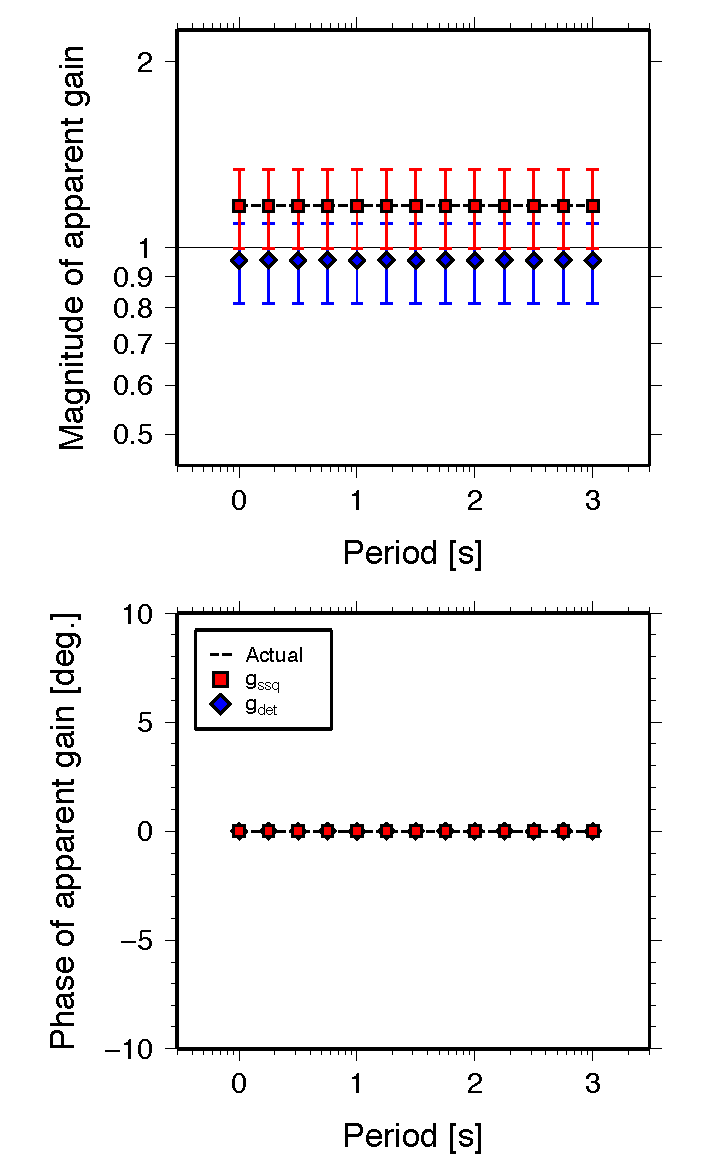
\includegraphics[scale=\plotmtrespscale]{\figdir/lyr11a_d10a_syn0203_gaina_magphs.pdf}
		\label{fig:appgain_example_1d}
	}
	\subfigure[]{
		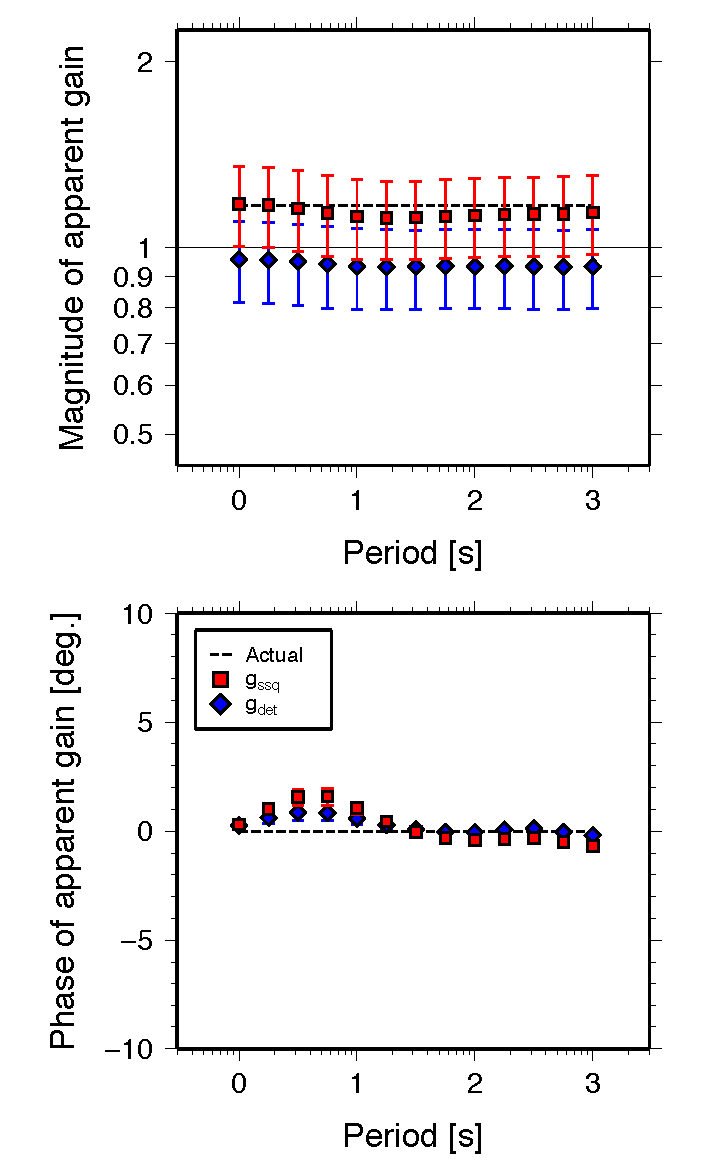
\includegraphics[scale=\plotmtrespscale]{\figdir/m02a-lyr11a_cb12-h0a2a-d05a-t01a_dr-e43n42_cb1X_loc-regi0_c-s40k-p0p0-pp1_d13a_syni0203_gaina_magphs.pdf}
		\label{fig:appgain_example_3d}
	}
	\caption[Example of apparent gains from 1D and 3D data]{Det (diamonds) and ssq (squares) apparent gains from (a) the 1D data and (b) station \texttt{syn08} in the 3D data. The distortion parameters with an SD of 0.3 are applied to both 1D and 3D datasets. 
	A synthetic site gain (dashed line) of 1.20 was applied at this station.}
	\label{fig:appgain_example}
\end{figure}

%% ==== Apparent gains
First, we show the examples of the apparent gains from the 1D data and 3D data at the station \texttt{syn08}. These data are distorted with the distortion parameters $\gtes$ is $(1.20, 0.11, -0.37, 0.49)$ (Figure \ref{fig:appgain_example}). 
%
As proven, the apparent gains from 1D data are real-valued and frequency independent. The apparent ssq gain accurately estimates the synthetic site gain, while the apparent det gain, here, is biased downward because of shear and splitting parameters (Figure \ref{fig:appgain_example_1d}). 
%
In the 3D case, the apparent gains show frequency dependent features and become weakly complex-valued number due to the inductive effect of the underlying 3D heterogeneity (Figure \ref{fig:appgain_example_3d}). 
%
However, the apparent ssq gain still agrees with the synthetic site gain within the uncertainty. As with the 1D example, the apparent det gain is biased downward by the distortion parameters. 
%
Note that the error bars (in Figure \ref{fig:appgain_example}) are derived from the standard error obtained from averaging the det and ssq impedances (Figure \ref{fig:resp3d_avg_distorted}). 
Therefore, if the distortion is very intense, the apparent gains will be less constrained.



%% ==== 
%\begin{itemize}
%\item
The apparent det and ssq gains as a function of period from the 3D datasets distorted with the distortion parameters with an SD of 0.3 are shown in Figure \ref{fig:appgain_3d_distorted}.
The apparent gains have a combination of the frequency dependence and independence.
The frequency-independent feature is upto the site gain contained at each station, while the frequency-dependent feature strongly depends on how strong the inductive effect of the underlying 3D structure is.



%% ==== gssq 3-D individual all 
\begin{figure}[t]
	\centering
	\subfigure[]{
		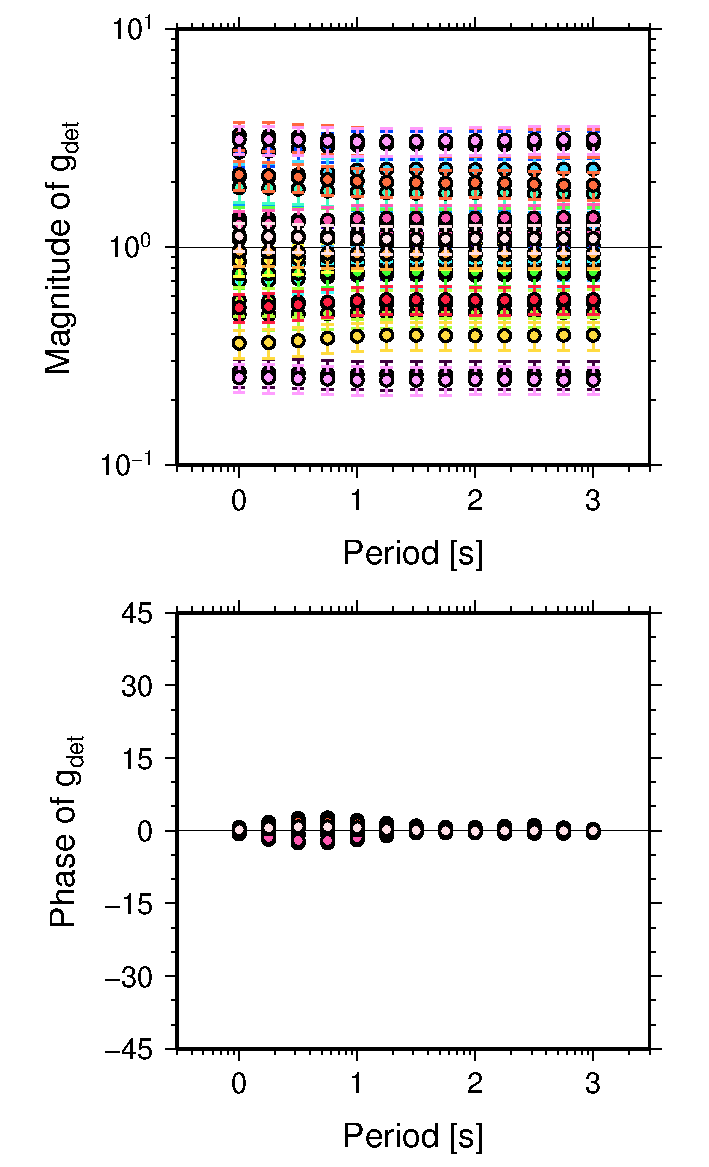
\includegraphics[scale=\plotmtrespscale]{\figdir/m02a-lyr11a_cb12-h0a2a-d05a-t01a_dr-e43n42_cb1X_loc-regi0_c-s40k-p0p0-pp1_d13a_distorted-sd3a-gtes_gdet_magphs.pdf}
		\label{fig:appgain_3d_distorted_gdet}
	}
	\subfigure[]{
		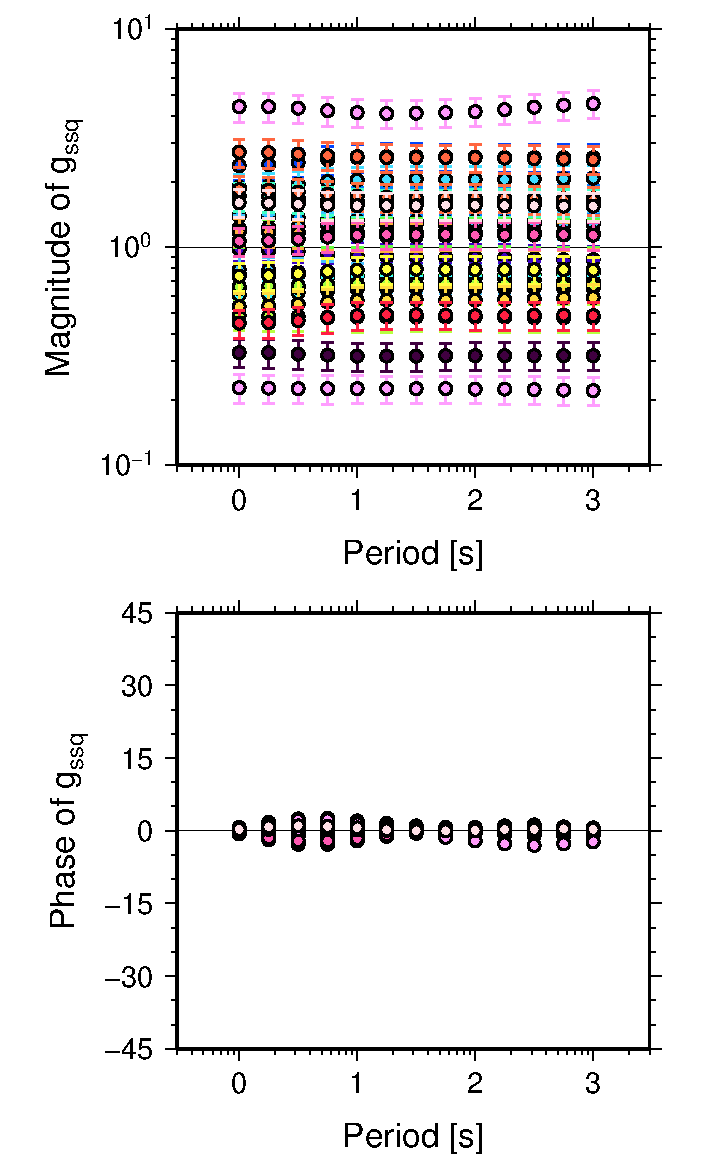
\includegraphics[scale=\plotmtrespscale]{\figdir/m02a-lyr11a_cb12-h0a2a-d05a-t01a_dr-e43n42_cb1X_loc-regi0_c-s40k-p0p0-pp1_d13a_distorted-sd3a-gtes_gssq_magphs.pdf}
		\label{fig:appgain_3d_distorted_gssq}
	}
	\caption[Apparent det and ssq gains from 3D dataset]{The apparent (a) det and (b) ssq gains derived from the 3D example, where a set of distortion parameters with an SD of 0.3 was applied.}
	\label{fig:appgain_3d_distorted}
\end{figure}

%% ==== Mean apparent gains
%\item 
However, to yield the more meaningful interpretation of them,
we calculate the mean apparent ssq and det gains using Eqs \eqref{eq:gdet_mean_def} and \eqref{eq:gssq_mean_def}. 
%\item 
To validate the mean apparent gains, we also define the percentage difference between the mean apparent gains (Eqs \ref{eq:gdet_mean_def} and \ref{eq:gssq_mean_def}) and the synthetic site gain $\gainpi$:
	\begin{equation}
		\mathcal{P}(\gssqimean) = \frac{\gssqimean - \gainpi}{\gainpi} \times 100\%
	\end{equation}	
	\begin{equation}
		\mathcal{P}(\gdetimean) = \frac{\gdetimean - \gainpi}{\gainpi} \times 100\%.
	\end{equation}
%\end{itemize}

%% Mean apparent gain 1D
%\begin{itemize}
%	\item
	From the 1D dataset, the mean apparent ssq gain correctly estimates the synthetic site gain in the data as confirmed by the zero percentage difference (Figure \ref{fig:appgain_1d_site}).
	Conversely, the mean apparent det gain would be either the overestimate or the underestimate of the site gain depending on the galvanic distortion strength, which could be pointed out by the local distortion indicator at individual sites (Figures \ref{fig:gamma_1d_site} and \ref{fig:gamma_3d_site}). This is because the det impedance is affected by the shear and splitting parameters.
	If the distortion at sites is stronger than average, the mean apparent det gain will be an underestimate (e.g., \texttt{syn01}, \texttt{syn03}, \texttt{syn09}). On the contrary, if the distortion at sites is weaker than average, the mean apparent det gain will be an overestimate (e.g., \texttt{syn04}, \texttt{syn05}).
	Note that error bars in this figure are derived from the error propagation rule when calculating Eqs. \eqref{eq:gdet_mean_def} and \eqref{eq:gssq_mean_def}.
	Although the mean apparent det gain agrees with the actual value within the uncertainty range, the mean apparent ssq gain is sitll the favorable choice.
%\end{itemize}

%% Mean 3D
%\redb{Mean 3D}
%\begin{itemize}
%\item
As shown before, the inductive effect from 3D structure can cause the frequency-dependent variation in the apparent gains (Figure \ref{fig:appgain_1d_site}). It may result in some error in estimating the site gain with the mean apparent gain. 
For instance, the mean apparent ssq gains from the stations over the conductive structure (e.g., \texttt{syn07}, \texttt{syn19}) underestimate the synthetic site gains, i.e., less than the actual value (Figure \ref{fig:appgain_3d_site}), as seen from the negative percentage difference.
On the contrary, if the stations are located over the resistive structure (e.g., \texttt{syn04}, \texttt{syn09}), the mean apparent gain is overestimated.
%
Despite of this, the estimate of site gain from the mean apparent ssq gain still agrees with the synthetic values within the statistical uncertainty.
%
%It should be noted that these errors also occur with the apparent det gain, but they are better observed from the apparent ssq gain because the ssq impedance is less sensitive to the galvanic distortion.
%\end{itemize}

%% ==== Concluding paragraph
%\begin{itemize}
%	\item \red{concluding paragraph}
%	\item 
	It is believed that the site gain is undeterminable without other independent geophysical data \citep[e.g.,][]{groom1993a, bibby2005a}.
%	\item 
	From the theoretical derivation and the synthetic examples, the apparent ssq gain is shown to be the promising parameter for the site gain estimation. 
	It is also important to note that this information can be gleaned from MT data alone.
	This parameter would help correcting the magnitude of MT impedances.	
%\end{itemize}

%% ==== App gain 1-D: Percentage difference
\begin{figure}[t]
	\centering
	\subfigure[]{
		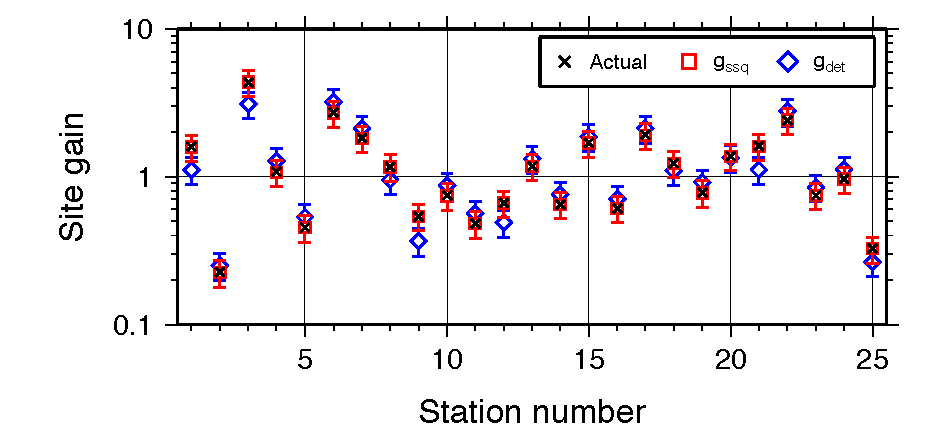
\includegraphics[scale=\plotdindmeanscale]{\figdir/lyr11a_n25_d13a_distorted-sd3a-gtes_gaina_est.pdf}
		\label{fig:appgain_1d_site_estimated}
	}
	\subfigure[]{
		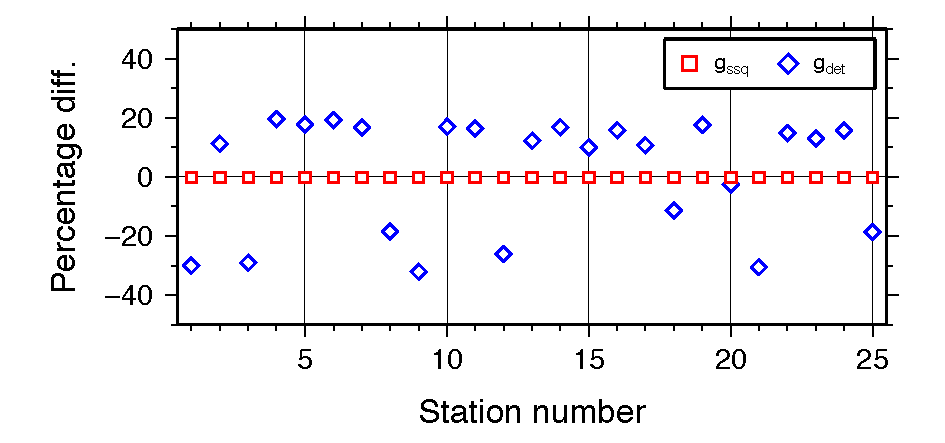
\includegraphics[scale=\plotdindmeanscale]{\figdir/lyr11a_n25_d13a_distorted-sd3a-gtes_gaina_est_diffp.pdf}
		\label{fig:appgain_1d_site_pdiff}
	}
	\caption[Comparison of the actual and the mean apparent gains from 1D dataset]{(a) Comparison of actual site gains (crosses) with the mean apparent det (diamonds) and ssq (squares) gains from the 1D example, where a set of distortion parameters with an SD of 0.3 was applied. (b) Percentage difference between the mean apparent gains and the actual site gains}
	\label{fig:appgain_1d_site}
\end{figure}

%% ==== App gain 3-D: Percentage difference
\begin{figure}[t]
	\centering
	\subfigure[]{
		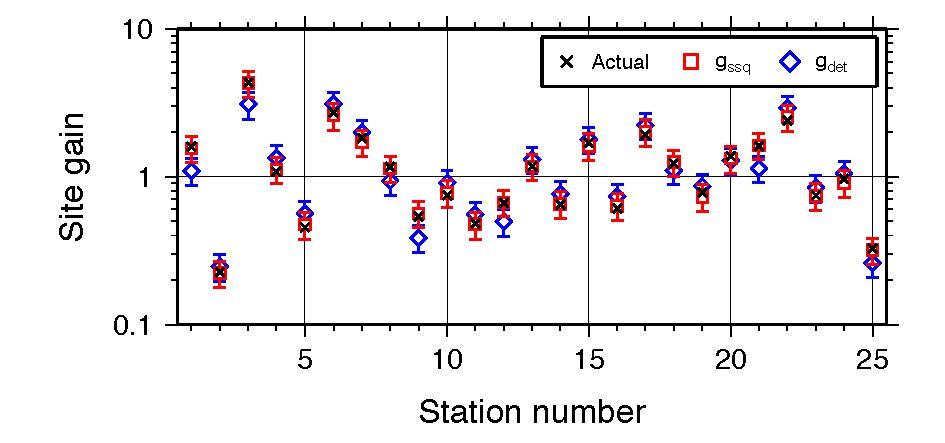
\includegraphics[scale=\plotdindmeanscale]{\figdir/m02a-lyr11a_cb12-h0a2a-d05a-t01a_dr-e43n42_cb1X_loc-regi0_c-s40k-p0p0-pp1_d13a_distorted-sd3a-gtes_gaina_est.pdf}
		\label{fig:appgain_3d_site_estimated}
	}
	\subfigure[]{
		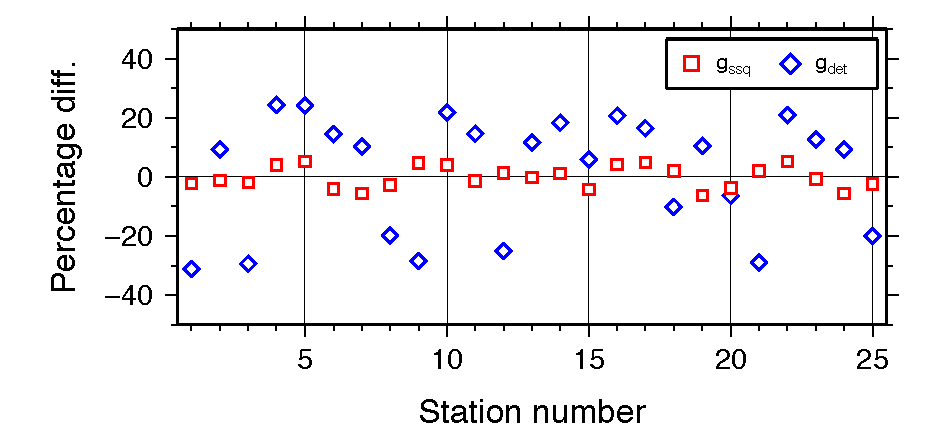
\includegraphics[scale=\plotdindmeanscale]{\figdir/m02a-lyr11a_cb12-h0a2a-d05a-t01a_dr-e43n42_cb1X_loc-regi0_c-s40k-p0p0-pp1_d13a_distorted-sd3a-gtes_gaina_est_diffp.pdf}
		\label{fig:appgain_3d_site_pdiff}
	}
	\caption{Same as Figure \ref{fig:appgain_1d_site} for the 3D example}
	\label{fig:appgain_3d_site}
\end{figure}
